\section{Массивы, векторы, связные списки. Устройство, основные операции, способы реализации}

\subsection{Массив}
\begin{definition}
    \textbf{Массив} - базовая структура данных - набор однотипных элементов, расположенных в памяти последовательно друг за другом.
\end{definition}
Пояснять тут больше нечего...

\subsection{Вектор}

\begin{definition}
    \textbf{Вектор} - структура данных, являющаяся надстройкой над массивом и поддерживающая следующие операции:
    \begin{itemize}
        \item Доступ к элементу; 
        \item Вставка элемента;
        \item Удаление элемента;
        \item Поиск.
    \end{itemize}
\end{definition}
\subsubsection{Устройство вектора}
Вектор содержит в себе динамический массив размера $capacity$. Текущее заполнение этого массива описывается параметром $size$.

Когда $size$ достигает определённого размера относительно $capacity$(об этом поговорим чуть позже), происходит перевыделение памяти: либо выделяется блок памяти размером поменьше, либо размером побольше - и туда перемещается $size$ элементов массива. Одновременно с этим меняется и $capacity$.

\subsubsection{Изменение $capacity$ в векторе}
Существует две стратегии изменения $capacity$:
\begin{itemize}
    \item Аддитивная: $capacity = oldCapacity + \Delta$. При этом $\Delta$ задаётся либо по умолчанию, либо в момент создания вектора.
    \item Мультипликативная: $capacity = coef * oldCapacity$. При этом $coef$ задаётся либо по умолчанию, либо в момент создания вектора.
\end{itemize}

\subsubsection{Условие изменения $capacity$ в векторе}
Здесь вволится следующая величина:
$$
loadFactor = \frac{size}{capacity}
$$
\begin{equation*}

\textbf{Если выбрана аддитивная стратегия:}

    \begin{cases}
        if (loadFactor \geq 0.8) \Rightarrow while(loadFactor \geq 0.8) capacity := capacity + \Delta;
    \end{cases}
    
\textbf{Если выбрана мультипликативная стратегия:}

    \begin{cases}
    if (loadFactor \leq \frac{1}{coef^2}) \Rightarrow \text{обрезаем память} \\
    if (loadFactor \geq 0.8) \Rightarrow \text{Перевыделяем память}\\
    \end{cases}
\end{equation*}

\subsubsection{Оценки операций с вектором}
\begin{tabular}{|p{2.5cm}|p{3.5cm}|p{3.5cm}|p{3.5cm}|}
\hline
     & Лучший случай & Средний случай&Худший случай \\
\hline
    Доступ & $O(1)$ & $O(1)$ & $O(1)$\\
\hline
    Вставка & $Amort(O(1))$ [вставка в конец]& $O(n)$ [вставка не в конец] & $O(n)$  [вставка в начало]\\
\hline
    Удаление & $Amort(O(1))$ [удаление с конца]& $O(n)$ [удаление не из конца]& $O(n)$ [удаление первого элемента]\\
\hline
    Поиск & $O(1)[искомый - первый]$ & $O(n)$ [искомый - не первый] & $O(n)$ [искомый - последний]\\
\hline
\end{tabular}
\subsubsection{Резюме}
\begin{tabular}{cp{10cm}}
    Достоинства: &
        \begin{equation*}
            \begin{cases}
                \text{Минимальный } overhead;\\
                \text{Простота реализации};\\
                \text{Быстрый доступ к элементам коллекции}.
            \end{cases}
        \end{equation*} \\
    Недостатки:&  
        \begin{equation*}
            \begin{cases}
                \text{Необходимо иметь нефрагментированную память;}\\
                \text{При большой загрузке долгое перевыделение памяти.}\\
            \end{cases}
        \end{equation*} 
\end{tabular}

\textbf{Используется в задачах, где необходим \textit{гарантированно} быстрый доступ к данным}.
\newpage
\subsection{Связный список}
\begin{definition}
    \textbf{Связный список} - структура данных, в которой каждый элемента содержит указатель на следующий элемент (случай односвязного списка) или и на следующий, и на предыдущий (двусвязный список).
\end{definition}

\begin{figure}[ht]
    \centering
    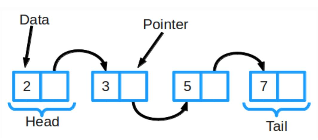
\includegraphics[scale=1]{List.png}
    \caption{Односвязный список}
    \label{fig:g}
\end{figure}

\subsubsection{Основные операции над списками}
\begin{itemize}
        \item Доступ к элементу; 
        \item Вставка элемента;
        \item Удаление элемента;
        \item Поиск.
\end{itemize}

\subsubsection{Оценка операций}
\begin{tabular}{|p{3cm}|p{3cm}|p{3cm}|p{3cm}|}
\hline
     & Лучший случай & Средний случай&Худший случай \\
\hline
    Доступ & $O(1)$ & $O(n)$ & $O(n)$\\
\hline
    Вставка (\textbf{если знаем}, куда вставлять) & $O(1)$ [вставка в конец]& $O(1)$  & $O(1)$  \\
\hline
    Удаление (\textbf{если знаем}, откуда удалять) & $O(1)$ & $O(1)$ & $O(1)$\\
\hline
    Поиск & $O(1)[искомый - первый]$ & $O(n)$ [искомый - не первый] & $O(n)$ [искомый - последний]\\
\hline
\end{tabular}

\subsection{Резюме}
\begin{tabular}{cp{10cm}}
    Достоинства: &
        \begin{equation*}
            \begin{cases}
                \text{Быстрое удаление};\\
                \text{Быстрая вставка};\\
                \text{Нет ограничений на фрагментацию памяти}.
            \end{cases}
        \end{equation*} \\
    Недостатки:&  
        \begin{equation*}
            \begin{cases}
                \text{Довольно приличный }overhead;\\
                \text{Долгий доступ к элементая коллекции.}\\
            \end{cases}
        \end{equation*} 
\end{tabular}

\textbf{Используется в задачах, где необходимы \textit{гарантированно} быстрые добавление и удаление узлов}.